\documentclass[11pt]{article}

\usepackage{fullpage}
\usepackage{url}
\usepackage{mathtools}
\usepackage{graphicx}
\usepackage{listings}
\usepackage{color}

\definecolor{dkgreen}{rgb}{0,0.6,0}
\definecolor{gray}{rgb}{0.5,0.5,0.5}
\definecolor{mauve}{rgb}{0.58,0,0.82}

\lstset{frame=tb,
  aboveskip=3mm,
  belowskip=3mm,
  showstringspaces=false,
  columns=flexible,
  basicstyle={\small\ttfamily},
  numbers=none,
  numberstyle=\tiny\color{gray},
  keywordstyle=\color{blue},
  commentstyle=\color{dkgreen},
  stringstyle=\color{mauve},
  breaklines=true,
  breakatwhitespace=true,
  tabsize=3
}

\begin{document}
\thispagestyle{empty}
\parindent 0pt
\vfill
\large

\begin{center}
\LARGE{\bf \textsf{CS246: Mining Massive Data Sets}} \\*[4ex]
\end{center}

{\Large
\textbf{Assignment number:} 2
\vfill
\vfill

Fill in and include this cover sheet with each of your assignments. It is an honor code
violation to write down the wrong time. Assignments and code are due at 5:00 PM on Scoryst and SNAP respectively. Failure to include the coversheet with you assignment will
be penalized by 2 points.
Each student will have a total of \textit{two} free late periods. \textit{One late period expires at the start of
each class}. (Assignments are due on Thursdays, which means the first late period expires on
the following Tuesday at 5:00 PM.) Once these late periods are exhausted, any assignments
turned in late will be penalized 50\% per late period. However, no assignment will be accepted
more than one late period after its due date. (If an assignment is due to Thursday then we
will not accept it after the following Thursday.)
\vfill
\vfill
{\Large
\textbf{Your name:} \underline{Priyank Mathur} \\
\textbf{Email:} \underline{priyankm@stanford.edu} \textbf{SUNet ID:} \underline{priyankm}\\*[2ex] }
Collaborators: \underline{Emrah Budur, Shundan Xiao, Dibyajyoti Ghosh, Arkajyoti Misra} \\
\vfill

\vfill

I acknowledge and accept the Honor Code.\\*[3ex]
\bigskip
\textit{(Signed)} \underline{Priyank Mathur}
% If you are not printing this document out, just type your initials above

\vfill
\vfill

\pagebreak[4]
\section*{Answer to Question 1.a}

Let the cosine similarity of vectors $u$ and $v$ be represented as 
$$ cos(u, v) = \frac{ \sum_{i} u_i * v_i }{||u|| * ||v||} $$

Let a row of a matrix be represented as $R(i, :)$ and a column as $R(:, j)$.\\

Now, consider the matrix calculated as $T = R^TR$, which will be an $n \times n$ matrix with each element as -
$$T_{1,1} = R(:, 1) R(:, 1)$$
$$T_{1,2} = R(:, 1) R(:, 2)$$
$$T_{3,2} = R(:, 3) R(:, 2)$$
\begin{center} {\dots} \end{center}

We see that this matrix is symmetrical and each element represents a dot product between 2 columns (movies) of matrix R. These elements are also the numerators in the cosine similarity we defined above. \\

Let matrix $Q^{\frac{1}{2}}$ represent the element wise square root of a matrix $Q$. We know that matrices P and Q are diagonal matrices and inverting a diagonal matrix is equivalent to dividing 1 by each of its non-zero elements, i.e.

\[
\begin{bmatrix}
    x_{11}   & 0 & 0 & \dots &0 \\
    0   & x_{22} & 0 & \dots & 0 \\
    \hdotsfor{5} \\
    0  & 0 & 0 & \dots & x_{nn}
\end{bmatrix}^{-1}
=
\begin{bmatrix}
    1/x_{11}       & 0 & 0 & \dots &0 \\
    0  & 1/x_{22} & 0 & \dots & 0 \\
    \hdotsfor{5} \\
    0   & 0 & 0 & \dots & 1/x_{nn}
\end{bmatrix}
\]

where $x_{ii}$ are the magnitudes of rows or columns in R. \\

We know the following about any diagonal matrix X:

\[
\begin{bmatrix}
    x_{11}   & 0 & 0 & \dots &0 \\
    0   & x_{22} & 0 & \dots & 0 \\
    \hdotsfor{5} \\
    0  & 0 & 0 & \dots & x_{nn}
\end{bmatrix} \times
\begin{bmatrix}
	a_{11} & a_{12} & \dots  & a_{1n} \\
    a_{21} & a_{22} & \dots  & a_{2n} \\
    \vdots & \vdots & \vdots & \vdots \\
    a_{n1} & a_{n2} & \dots  & a_{nn}
\end{bmatrix}
=
\begin{bmatrix}
	x_{11}a_{11} & x_{11}a_{12} &  \dots  & x_{11}a_{1n} \\
    x_{22}a_{21} & x_{22}a_{22} & \dots  & x_{22}a_{2n} \\
    \vdots & \vdots & \vdots & \vdots \\
    x_{nn}a_{n1} & x_{nn}a_{n2} & \dots  & x_{nn}a_{nn}
\end{bmatrix}
\]

and
\[
\begin{bmatrix}
	a_{11} & a_{12} & \dots  & a_{1n} \\
    a_{21} & a_{22} & \dots  & a_{2n} \\
    \vdots & \vdots & \vdots & \vdots \\
    a_{n1} & a_{n2} & \dots  & a_{nn}
\end{bmatrix} \times
\begin{bmatrix}
    x_{11}   & 0 & 0 & \dots &0 \\
    0   & x_{22} & 0 & \dots & 0 \\
    \hdotsfor{5} \\
    0  & 0 & 0 & \dots & x_{nn}
\end{bmatrix}
=
\begin{bmatrix}
	x_{11}a_{11} & x_{22}a_{12} &  \dots  & x_{nn}a_{1n} \\
    x_{11}a_{21} & x_{22}a_{22} & \dots  & x_{nn}a_{2n} \\
    \vdots & \vdots & \vdots & \vdots \\
    x_{11}a_{n1} & x_{22}a_{n2} & \dots  & x_{nn}a_{nn}
\end{bmatrix}
\] \\

Hence, the matrix $[Q^{\frac{1}{2}}]^{-1} T [Q^{\frac{1}{2}}]^{-1}$ represents a matrix where each element has numerator representing dot product of 2 columns and denominator is the product of magnitudes of same 2 columns. Therefore, each each element is cosine similarity between 2 columns. \\

$$S_I = [Q^{\frac{1}{2}}]^{-1} R^TR [Q^{\frac{1}{2}}]^{-1}$$

Similarly, consider $$U = RR^T$$ which will be a $m \times m$ matrix with numerators representing the dot products between any 2 users. By using the results from above, we can say that

$$S_U = [P^{\frac{1}{2}}]^{-1} RR^T [P^{\frac{1}{2}}]^{-1}$$

\pagebreak[4]
\section*{Answer to Question 1.b}

$r_{u,s} = \sum_{x \in users} cos(x, u) \times R_{x,s}$ represents the recommendation method.\\
e.g.

$$r_{1,1} = cos(1,1)R_{11} + cos(1,2)R_{21} + \hdots + cos(1,m)R_{m1}$$

From previous question, we know that $$S_U = [P^{\frac{1}{2}}]^{-1} RR^T [P^{\frac{1}{2}}]^{-1}$$ is an $m \times m$ symmetric matrix representing the cosine similarity for all users vs. all other users. So, 
$$r_{1,1} = S_{11}R_{11} + S_{12}R_{21} + \hdots + S_{1m}R_{m1} = r_{1,1}$$

Then let $A = S_UR$, where
$$A_{1,1} = S_{11}R_{11} + S_{12}R_{21} + \hdots + S_{1m}R_{m1} = r_{1,1}$$
$$A_{1,2} = S_{11}R_{12} + S_{12}R_{22} + \hdots + S_{1m}R_{m2} = r_{1,2} $$
$$A_{1,3} = S_{11}R_{13} + S_{12}R_{23} + \hdots + S_{1m}R_{m3} = r_{1,3} $$
\begin{center} {\dots} \end{center}

Therefore, each element of matrix $A$ represents the metric $r$ for that user.
$$\Gamma_U = S_UR = [P^{\frac{1}{2}}]^{-1} RR^T [P^{\frac{1}{2}}]^{-1}R$$ which is an $m \times n$ matrix.\\

Using the same approach as above, $$\Gamma_I = RS_I = R[Q^{\frac{1}{2}}]^{-1} R^TR [Q^{\frac{1}{2}}]^{-1}$$ which is an $m \times n$ matrix.

\pagebreak[4]
\section*{Answer to Question 1.c}
$$T = RR^T$$
From part 1.a we know that $T$ is a symmetric matrix with each element representing the dot product of 2 rows of the matrix $R$. This can also be thought of as each element representing the dot product of 2 users.\\

Since each element in $R$ is either 0 or 1 represents an edge in the graph, the dot product of 2 user rows represents the degree of overlap between the 2 vectors.\\

The entries along the main diagonal of $T$,  ($T_{ii}$), represent the overlap between the user and itself. In other words, this represents the out degree of that users node in the bipartite user-to-item graph.\\

The other entries of $T$,  ($T_{ij}$), represent the overlap between a user and another user. In other words, this represents the number of items that both these users liked, i.e. the number of that item nodes in the bipartite user-to-item graph that both users are connected to.

\pagebreak[4]
\section*{Answer to Question 1.d}

Code at the end of the file.

\subsection*{Top movies using user-user similarity}
\begin{tabular}{ l c r }
"FOX 28 News at 10pm" & 908.480053476\\
"Family Guy" & 861.175999287\\
"2009 NCAA Basketball Tournament" & 827.601295474\\
"NBC 4 at Eleven" & 784.781958904\\
"Two and a Half Men" & 757.601118102\\
\end{tabular}

\subsection*{Top movies using item-item similarity}
\begin{tabular}{ l c r }
"FOX 28 News at 10pm" & 31.3647016783\\
"Family Guy" & 30.0011417989\\
"NBC 4 at Eleven" & 29.3967977734\\
"2009 NCAA Basketball Tournament" & 29.2270015615\\
"Access Hollywood" & 28.9712776741\\
\end{tabular}\\
\\

\includegraphics*{q1cc}\\

From the above graph, we can not adequately distinguish between the performance of the two methods. The rate of increase of true positive rate for $k \in [1,19]$ for both the methods is comparable.

\pagebreak[4]
\section*{Answer to Question 2a}

\subsection*{1.}
We know that $C =A^TA$. We can prove C is symmetric by the following argument - \\

$C_{ij} = (A^T  A)_{ij} \\
= \sum_k [ A^T_{ik}  A_{kj} ] \\
= \sum_k [ A_{ki}  A^T_{jk} ]$ as $A_{ij} = A^T_{ji} \\
= \sum_k [ A^T_{jk}  A_{ki} ] \\
= (A^T  A)_{ji}\\
= C_{ji}$ \\

Similarly, $K = AA^T$ is also symmetric since $K_{ij} = K_{ji}$ by the above argument.\\

$K_{ij} = (A  A^T)_{ij} \\
= \sum_k [ A_{ik}  A^T_{kj} ] \\
= \sum_k [ A^T_{ki}  A_{jk} ]$ as $A_{ij} = A^T_{ji} \\
= \sum_k [ A_{jk}  A^T_{ki} ] \\
= (A  A^T)_{ji}\\
= K_{ji}$ \\

We know that -
\begin{itemize}
\item $A = USV^T$.
\item $C$ is a real, symmetric, and square $n \times n$ matrix which can be decomposed as 
\begin{equation}
C=Q \Sigma Q^T
\end{equation}	
where  $Q$ is an orthogonal matrix containing the eigenvectors of $C$ as its columns and $\Sigma$ contains the eigenvalues of $C$.\\
\end{itemize} 
$C = A^T A = (USV^T)^TUSV^T \\
= V S^T U^T U S V^T  \\
= V S^T S V^T  \hspace{30 mm}$ Since $U^T U = I\\
= V \Sigma V^T$ \hspace{30 mm} where $\Sigma = S^T S$\\

Comparing the result with (1), we know that $\Sigma$ contains the eigen values of $C$ and $V$ has the eigenvectors of $C$.\\

$\Sigma = S^T S$ is an $n \times n$ matrix where $S$ is a diagonal matrix containing $\sigma_{kk}$ which are the singular values of $A$. Since $n \gg m$ we will only have $m$ non zero eigenvalues.\\

Therefore $\Sigma$ is also a diagonal matrix with eigenvalues $(\lambda)$ as -
$$\lambda_{kk} = \sigma_{kk}^2$$ for $k \leq m$ and 0 for $k > m$. The matrix $V$ has the eigenvectors for matrix $C$ in its columns.\\

Using the same logic for $K = AA^T$, we get -

$K = A A^T = USV^T(USV^T)^T \\
= U S V^T V S^T U^T \\
= U S S^T U^T  \hspace{30 mm}$ Since $V^T V = I\\
= U \Sigma U^T$ \hspace{30 mm} where $\Sigma = S S^T$\\

Therefore $\Sigma$ is also a matrix with eigenvalues of K $(\lambda)$ as -
$$\lambda_{kk} = \sigma_{kk}^2$$ for $k \leq m$. The matrix $U$ has the eigenvectors for matrix $K$ in its columns.\\

\pagebreak[4]
\subsection*{2.}

We should use $K$ for computing the singular values of A using matrix $K$'s eigenvalue decomposition. $K$ is a $m \times m$ matrix, and in this case $n \gg m$. Since the operation of calculating eigenvalues is expensive $O(d^3)$, we can use the smaller matrix $K$ to get its eigenvalue decomposition and then calculate the singular values from it by simply using the square root of each eigenvalue.

\pagebreak[4]
\subsection*{3.}

In part 3.a, we saw that matrix $C$ has eigenvectors as columns of matrix $V$ and eigenvalues as $S^T S$. That is
\begin{align*}
C = V S^T S V^T\\
\implies A^T A = V S^T S V^T
\end{align*}
Since $V^T = V^{-1}$ as $V$ is orthogonal
\begin{align*}
\implies A^T A = V S^T S V^{-1}\\
\implies A^T A V = V S^T S
\end{align*}

Here $S$ is a matrix containing singular values. We can obtain $S$ by taking the square root of each of the eigenvalues.\\

We can write each column of $V$ as
$$(A^TA) v_k = \lambda_k v_k$$ where $\lambda_k$ is the eigenvalue which is equal to $\sigma_k^2$, the singular value. Hence we can extract the right singular matrix $V$ and the singular values $S$ from the above equations.\\

To find $U$, we can solve the below equation
\begin{align*}
A = U S V^T = U S V^-1\\
\implies A V = U S
\end{align*}	

\pagebreak[4]
\subsection*{4.}

In part 3.a, we saw that matrix $K$ has eigenvectors as columns of matrix $U$ and eigenvalues as $S S^T$. That is
\begin{align*}
K = U S S^T U^T\\
\implies A A^T = U S S^T U^T
\end{align*}
Since $U^T = U^{-1}$ as $U$ is orthogonal
\begin{align*}
\implies A A^T = U S S^T U^{-1}\\
\implies A A^T U = U S S^T
\end{align*}

Here $S$ is a matrix containing singular values. We can obtain $S$ by taking the square root of each of the eigenvalues.\\

We can write for each column of $U$ as
$$(AA^T) u_k = \lambda_k u_k$$ where $\lambda_k$ is the eigenvalue which is equal to $\sigma^2$, the singular value. Hence we can extract the left singular matrix $U$ and the singular values $S$ from the above equations.\\

To find $V$, we can solve the below equation
\begin{align*}
A = U S V^T = U S V^-1\\
\implies A V = U S\\
\implies A V S^{-1} = U
\end{align*}	

\pagebreak[4]
\section*{Answer to Question 2b}
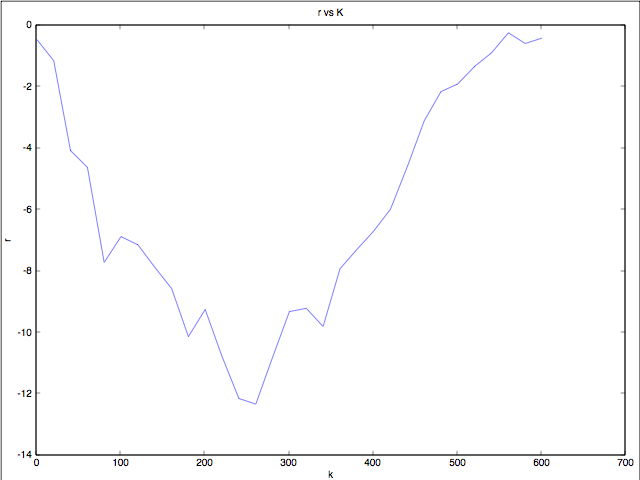
\includegraphics[scale=0.8]{q2err}

From the above curve we see that we achieve minimum r of -12.347 at k=261.\\

Code at the end of the file.
\pagebreak[4]
\section*{Answer to Question 2c}

\subsection*{1.}
To find $W$ that minimizes $||A-XW||_F^2$, we take its derivative w.r.t. W and solve
$$ \frac{\partial (A-XW)^T(A-XW)}{\partial W} = 0 $$
$$ \implies \frac{\partial (A^TA-2W^TX^TA-W^TX^TXW)}{\partial W} = 0 $$
$$ \implies \frac{\partial (A^TA-2W^TX^TA-W^TW)}{\partial W} = 0 $$

Solving, we get $W = X^T A$

\subsection*{2.}
By setting $X = \bar{U}$, we only consider the first $k$ singular vectors of $U$. From this, A can be reconstructed as 
$$A = \bar{U}\bar{S}\bar{V}^T$$

From part 1,
$$W = X^T A = \bar{U}^T \bar{U}\bar{S}\bar{V}^T$$
Since matrix $\bar{U}$ is orthogonal, we get

$$W = \bar{S}\bar{V}^T$$

\subsection*{3.}
$min_{X^TX = I_K} ||A-XW||_F^2$\\

Replacing $W = X^T A$ from part 1, we get

$$min_{X^TX = I_K} ||A-XX^T A||_F^2$$
$$ \implies min_{X^TX = I_K} ||A (I-XX^T)||_F^2$$

\pagebreak[4]
\section*{Answer to Question 3.a}
To prove -
$$\sum_{x \in S} || x - z ||^2 - \sum_{x \in S} || x - c(S)||^2 = |S| . || c(S) - z ||^2$$

We know that 
$$||u - v||^2 = (u - v)^T (u - v) = ||u||^2 + ||v||^2 - 2u.v$$

Let S be a set of n points $x_1, x_2 \hdots x_n$. Expanding LHS of the equation, we get -
$$ || x_1 - z ||^2 + || x_2 - z ||^2 + \hdots + || x_n - z ||^2$$ 
$$- || x_1 - c(S)||^2 - || x_2 - c(S)||^2 - \hdots - || x_n - c(S)||^2$$

$$ = ||x_1||^2 + ||z||^2 - 2x_1.z + ||x_2||^2 + ||z||^2 - 2x_2.z + \hdots + ||x_n||^2 + ||z||^2 - 2x_n.z$$
$$ - ||x_1||^2 - ||c(S)||^2 + 2x_1.c(S) - ||x_2||^2 - ||c(S)||^2 + 2x_2.c(S) + \hdots - ||x_n||^2 - ||c(S)||^2 + 2x_n.c(S)$$

$$ = n ||z||^2 - n ||c(S)||^2 + 2 c(S) (x_1 + x_2 + \hdots + x_n) - 2 z (x_1 + x_2 + \hdots + x_n)$$
We know that
$$c(S) = \frac{(x_1 + x_2 + \hdots + x_n)}{n}$$

\setcounter{equation}{0}
\begin{equation}
\implies  (x_1 + x_2 + \hdots + x_n) = n \times c(S)
\end{equation} 

Using (1), we get
$$ = n ||z||^2 - n ||c(S)||^2 + 2 n c(S).c(S)  - 2 n z c(S)$$
$$ = n ||z||^2 + n ||c(S)||^2 - 2 n z c(S)$$
$$ =  n . || c(S) - z ||^2 = |S| . || c(S) - z ||^2$$


\pagebreak[4]
\section*{Answer to Question 3.b}
From the previous part, we know that $$\sum_{x \in S} || x - z ||^2 - \sum_{x \in S} || x - c(S)||^2 = |S| . || c(S) - z ||^2$$

Here, if $z = c(S)$, 

\setcounter{equation}{0}
\begin{equation}\label{eq:simple}
\sum_{x \in S} || x - z ||^2 - \sum_{x \in S} || x - c(S)||^2 = 0
\end{equation}

If $z \neq c(S)$
$$|S| . || c(S) - z ||^2 > 0$$
\begin{equation}\label{eq:simple}
\implies \sum_{x \in S} || x - z ||^2 - \sum_{x \in S} || x - c(S)||^2 > 0
\end{equation}

From (1) and (2), we get
\begin{equation}\label{eq:simple}
\sum_{x \in S} || x - z ||^2 \geq \sum_{x \in S} || x - c(S)||^2 
\end{equation}

That is, distance of a set of points from a query point is minimum if the query point is the centroid of the set of data.\\

Let $C_{t1}, C_{t2} \hdots C_{tk}$ be the $k$ clusters at end of $t^{th}$ iteration with $c_{t1}, c_{t2} \hdots c_{tk}$ centroids. Similarly for iteration $(t+1)$, clusters are $C_{(t+1)1}, C_{(t+1)2} \hdots C_{(t+1)k}$ with centroids $c_{(t+1)1}, c_{(t+1)2} \hdots c_{(t+1)k}$. \\

Let $Cost (C_1, C_2 \hdots C_k, c_1, c_2 \hdots c_k)$ represent the cost while using clusters $C_1, C_2 \hdots C_k$ and centroids as $c_1, c_2 \hdots c_k$.\\

Now, $$\phi = \sum_{x \in X} min_{c \in C} ||x-c||^2$$

We know 
\begin{itemize}
\item $||x-c||^2$ will be minimum when $x$ belongs to the cluster represented by centroid c.
\item In each iteration's step (2), a point is placed in the cluster of its nearest centroid. This reduces the error as per the definition of $\phi$ above, that is
\begin{equation}\label{eq:simple}
\begin{aligned}
Cost (C_{(t+1)1}, C_{(t+1)2} \hdots C_{(t+1)k}, c_{t1}, c_{t2} \hdots c_{tk}) \leq Cost (C_{t1}, C_{t2} \hdots C_{tk}, c_{t1}, c_{t2} \hdots c_{tk})
\end{aligned}
\end{equation}

\item In each iteration's step (3), the new centorid is calculated as the average of the cluster points, so it is closer to the data points within the cluster, also contributing by reducing error. We can see this by using equation (3) above, where z is the old centroid and c(S) is the new centroid.\\
\begin{equation}\label{eq:simple}
\begin{aligned}
Cost (C_{(t+1)1}, C_{(t+1)2} \hdots C_{(t+1)k}, c_{(t+1)1}, c_{(t+1)2} \hdots c_{(t+1)k}) \leq \\
Cost (C_{(t+1)1}, C_{(t+1)2} \hdots C_{(t+1)k}, c_{t1}, c_{t2} \hdots c_{tk})
\end{aligned}
\end{equation}

\end{itemize}

Therefore, iteration $(t+1)$ should have better or atleast as good cluster assignments as iteration $t$. \\

Hence, from (3), (4) and (5), we can deduce that $\phi^t \geq \phi^{t+1}$.


\pagebreak[4]
\section*{Answer to Question 3.c}
\setcounter{equation}{0}
Let $C_{t1}, C_{t2} \hdots C_{tk}$ be the $k$ clusters in $t^{th}$ iteration with $c_{t1}, c_{t2} \hdots c_{tk}$ centroids. Similarly for iteration $(t+1)$, clusters are $C_{(t+1)1}, C_{(t+1)2} \hdots C_{(t+1)k}$ with centroids $c_{(t+1)1}, c_{(t+1)2} \hdots c_{(t+1)k}$. \\

Let $Cost (C_1, C_2 \hdots C_k, c_1, c_2 \hdots c_k)$ represent the cost while using clusters $C_1, C_2 \hdots C_k$ and centroids as $c_1, c_2 \hdots c_k$.\\

We know that -
\begin{itemize}
\item From 3.a) that the distance of a set of points from a query point is minimum if the query point is the centroid of the set of data.
\item From 3.b) we know that the error function $\phi$ is a monotonically decreasing function, i.e. $\phi^t \geq \phi^{t+1}$.
\item For a fixed k, the global optimal cluster assignment for the data set will give us the lowest possible cost. 
\end{itemize}

Assume we break ties during cluster assignment consistently, for e.g. by assigning to cluster centroid with the lower id (index). Given these facts, for any data set and $k$ (number of clusters), there are only a finite number of cluster assignments. \\

As we saw in 3.b), step (2) and (3) of the k-means algorithm reduce the overall cost. Hence, cluster assignments will keep changing to reduce $\phi$.

\begin{equation}\label{eq:simple}
\begin{aligned}
Cost (C_{(t+1)1}, C_{(t+1)2} \hdots C_{(t+1)k}, c_{t1}, c_{t2} \hdots c_{tk}) \leq Cost (C_{t1}, C_{t2} \hdots C_{tk}, c_{t1}, c_{t2} \hdots c_{tk})
\end{aligned}
\end{equation} and
\begin{equation}\label{eq:simple}
\begin{aligned}
Cost (C_{(t+1)1}, C_{(t+1)2} \hdots C_{(t+1)k}, c_{(t+1)1}, c_{(t+1)2} \hdots c_{(t+1)k}) \leq \\
Cost (C_{(t+1)1}, C_{(t+1)2} \hdots C_{(t+1)k}, c_{t1}, c_{t2} \hdots c_{tk})
\end{aligned}
\end{equation}

This is continued until we do not modify the assignments anymore, since we either -
\begin{itemize}
\item reached an assignment state where each point is already assigned to its nearest centroid from previous iteration.
\item or we cycled through all possible cluster assignments and we reach the optimum cost in the last iteration.
\end{itemize}

At this iteration, using (1) and (2), we can say that \underline{$\phi$ converges} to the finite value corresponding to this optimal assignment state. Note that this optimal assignment is not guaranteed to be globally optimum.\\

Extending the same logic as above, we can argue that \underline{k-means algorithm will converge} either when -
\begin{itemize}
\item we reach an assignment state where each point is already assigned to its nearest centroid from previous iteration.
\item or we cycled through all possible cluster assignments and we reach the optimum state in the last iteration.
\end{itemize}

\pagebreak[4]
\section*{Answer to Question 3.d}

\textbf{Data distribution}
Let the actual data be present in the below format. There are 3 true circular clusters with the points lying on the circumference of the circle. In this setting, each circle will ideally have its centroid at the center of the circle. Let each of the 3 clusters have n points. Also for the sake of analysis, we will assume the radius (r) of the 3 circles to be 1.

We will also assume that the distance $G \gg K$
\\

Thus, the optimal cost is equal to -
$$\phi_{Opt} = 3 \times n^2 r = 3n^2$$
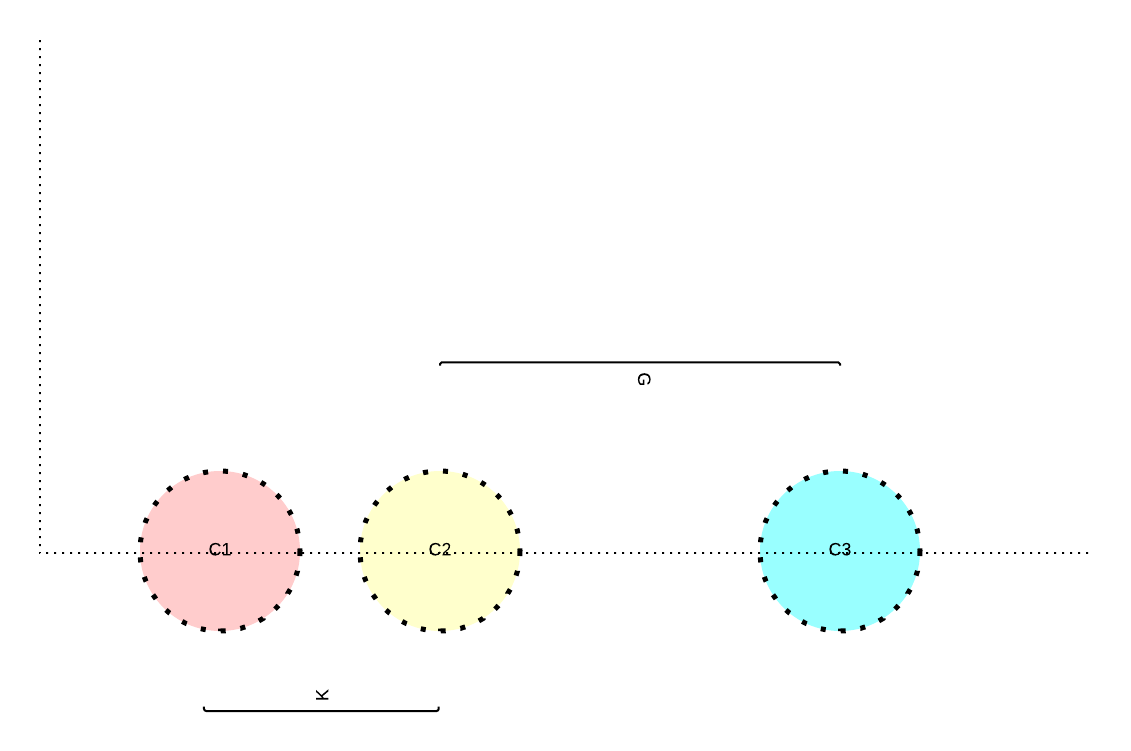
\includegraphics[scale=0.8]{q3_1} \\

Now, lets assume a bad initialization as shown in diagram below. The farthest cluster gets 2 centroid allocations.

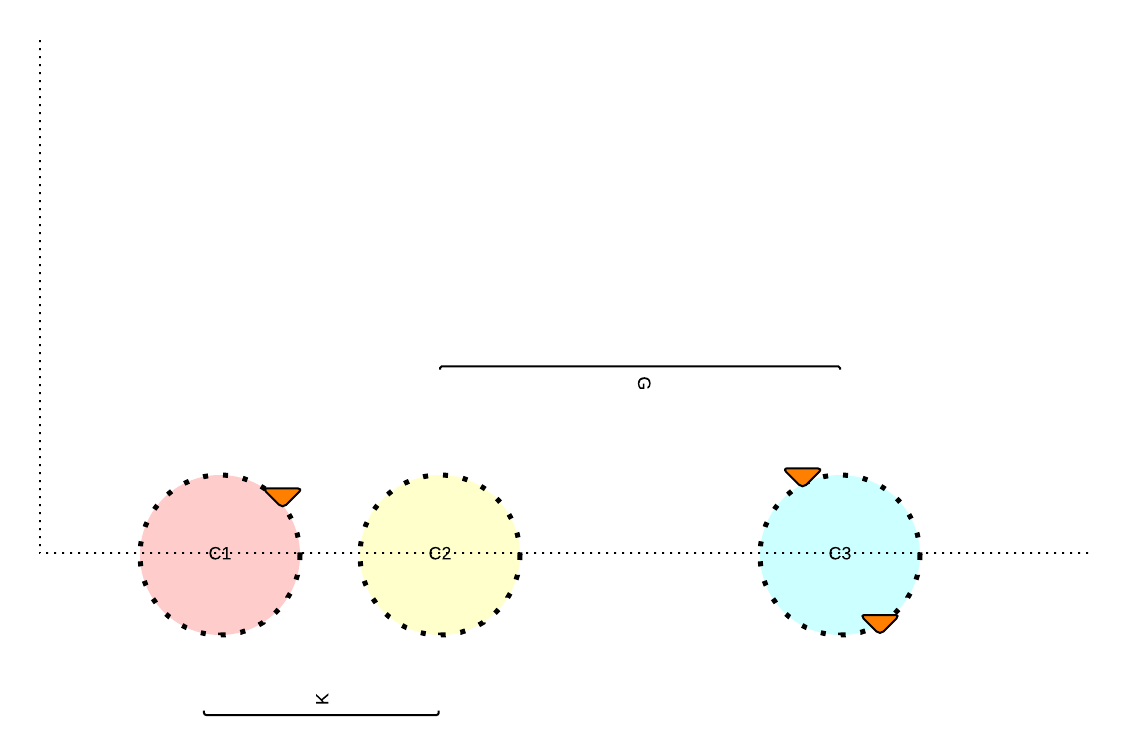
\includegraphics[scale=0.8]{q3_2} \\

In this case, the k-means algorithm will converge with the following cluster assignments.\\
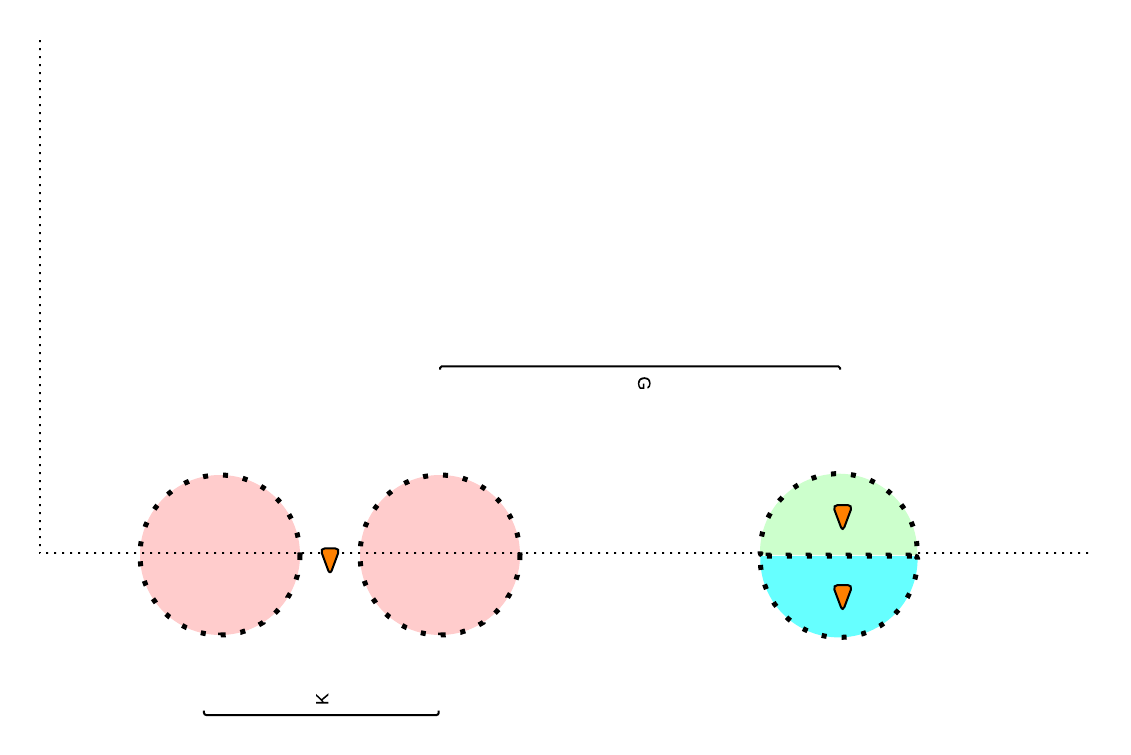
\includegraphics[scale=0.8]{q3_3} \\

From 3.a, we know that \\

$
\sum_{x \in S} || x - z ||^2 - \sum_{x \in S} || x - c(S)||^2 = |S| . || c(S) - z ||^2 \\ \\
\implies \sum_{x \in S} || x - z ||^2 = |S| . || c(S) - z ||^2 + \sum_{x \in S} || x - c(S)||^2
$ \\

where z are the centroids in the bad initialization. \\

Therefore, for cluster C1 and C2, the new cost will be
$$\phi_{C1} + \phi_{C2} = n^2 + n (\dfrac{K}{2})^2 + n^2 + n (\dfrac{K}{2})^2$$
$$\phi_{C1} + \phi_{C2} = 2n^2 + n \dfrac{K^2}{2} $$

Cluster 3 is actually divided into 2 new clusters and hence its cost will reduce, therefore the new cost for C3 is -
$$\phi_{C3} = n^2 - 2 \times \frac{n}{2} (\dfrac{4}{3\pi})^2$$
Since the centroid of a semi circle is located at $(0, \dfrac{4r}{3\pi})$.
$$\phi_{C3} = n^2 - n \dfrac{16}{9 \pi^2}$$

Therefore, total new cost = 
$$\phi_{new} = 2n^2 + n \dfrac{K^2}{2} + n^2 - n \dfrac{16}{9 \pi^2} $$
$$\implies \phi_{new} = 3n^2 + n (\dfrac{K^2}{2} - \dfrac{16}{9 \pi^2})  $$
$$\implies \phi_{new} = 3n^2 + n (\dfrac{K^2}{2} - 0.18)  $$

Hence, the ratio of costs is
$$ r = \dfrac{\phi_{new}}{\phi_{Opt}} = \dfrac{3n^2 + n (\dfrac{K^2}{2} - 0.18)}{3n^2}$$
$$ r = 1 + \frac{1}{3n} (\dfrac{K^2}{2} - 0.18)$$

We know that for true clusters C1 and C2 to be different, $K > 2 \times radius > 2$.

Hence the ratio $r$ is always greater than 1.\\

We can make $r$ arbitrarily greater than 1 by increasing distance $K$ and $G$, as long as $G \gg K$.

\pagebreak[4]
\section*{Answer to Question 4a}
Code at the end of the file.

\pagebreak[4]
\section*{Answer to Question 4b}
\includegraphics*{q4err}\\
As we can see, the cost decreases in each iteration till the algorithm converges. We also see that random initialization works much worse than clusters chosen in c2.txt.

\pagebreak[4]
\section*{Answer to Question 4c}
As we can see from the above graph, the random cluster initialization performs worse than using initial centroids as computed for c2.txt. We saw in question 3 that due to certain bad initialization, k-means can reach convergence at a sub optimal value which seems to be the case with c1.txt. 

Using initial centroids that are far away from each other gives us a higher chance of getting clusters that are governed by data distribution, since we get centroids that represent even the farthest points.\\

Change in cost $(\phi)$ for c1.txt $= \frac{459018805.0 - 623658084.0}{623658084.0} \times 100 = -26.39$\\

That is a decrease of 26.39$\%$.\\

Change in cost $(\phi)$ for c2.txt $= \frac{108545091.0 - 438745437.0}{438745437.0} \times 100 = -75.26$\\

That is a decrease of 75.26$\%$.\\

As we see, c2.txt performs much better job of decreasing the error.

\pagebreak[4]
\section*{Answer to Question 4d}

Top 5 words for document 2 are - \\
\begin{itemize}
\item instillation
\item methoxyfenozide
\item sodium-sensitive
\item post-infectious
\item teleological
\end{itemize}

\pagebreak[4]
\section*{Code for Q1}

\lstinputlisting[language=Python]{submission/snap/priyankm_hw2_q1.txt}


\pagebreak[4]
\section*{Code for Q2}

\lstinputlisting[language=Matlab]{submission/snap/priyankm_hw2_q2.txt}

\pagebreak[4]
\section*{Code for Q4}

\lstinputlisting[language=Java]{submission/snap/priyankm_hw2_q4.txt}

\end{document}
